\section{Electronic excitation by the recoil}\label{sec:19.2}

A silicon nucleus recoiling with \SI{100}{eV} moves at \SI{26}{km/s}, eighty times slower than the valence electrons at the Fermi velocity. A neutron calibration finds that such recoils leave on average 2.7 electron--hole pairs, an ionization yield of $0.102^{+0.034}_{-0.030}$~\cite[Table~II]{albakry2023first}. Yet a binary collision between the nucleus and a valence electron cannot create a single pair until the recoil carries about \SI{350}{eV}. The charge at \SI{100}{eV} must therefore come from processes that the binary picture leaves out, and these are the processes that set the charge signal of light dark matter, whose nuclear recoils in silicon stay below \SI{100}{eV} for masses under \SI{0.44}{GeV}. The question is which processes those are, and how much of the charge the Migdal effect of \cref{chap:12} already supplies.

\subsection{The binary electron--hole threshold}\label{sec:19.2-binary}

The recoiling ion is a projectile of the master formula, as the hot carrier of \cref{sec:18.1} was. It couples to the electron density through its screened charge, and the energy it hands to the electrons at momentum $\vect{k}$ is $\omega = \vect{k}\cdot\vect{v}_N - k^2/2M_\kappa \le kv_N$, with $v_N = q/M_\kappa$ the nuclear velocity after the kick. The stopping power \cref{eq:4.4-dEdx} contains this constraint as the upper limit $\omega \le kv_N$ of its inner integral; \cref{sec:19.3} evaluates that integral.

Consider first a free electron gas with the valence density of the crystal and a gap $\Eg$ added by hand. Its loss function vanishes outside the particle--hole continuum of \cref{sec:4.2}, which for $k > 2k_{\mathrm{F}}$ begins at $\omega_-(k) = k^2/2m_e - kv_{\mathrm{F}}$. An electron--hole pair needs $\omega \ge \Eg$, and the ion supplies at most $\omega = kv_N$. Both conditions hold at some $k$ only if the line $\omega = kv_N$ rises above $\omega_-(k)$ at an energy of at least $\Eg$. The line and the edge cross at $k = 2m_e(v_N + v_{\mathrm{F}})$, where $\omega = 2m_ev_N(v_N + v_{\mathrm{F}})$, and this is the largest energy the ion can deposit in one electronic excitation:
\begin{equation}
  \omega_{\mathrm{max}} = 2m_e v_N\,(v_N + v_{\mathrm{F}}) .
  \label{eq:19.2-transfer}
\end{equation}
The same number follows from a collision of two particles. In the rest frame of the heavy ion an electron moving against it at $v_{\mathrm{F}}$ approaches with speed $v_{\mathrm{F}} + v_N$ and is reflected with the same speed, and in the crystal frame it leaves with $v_{\mathrm{F}} + 2v_N$. Its kinetic energy rises by $\tfrac12 m_e[(v_{\mathrm{F}} + 2v_N)^2 - v_{\mathrm{F}}^2]$, which is \cref{eq:19.2-transfer}. The heavy ion acts as a moving wall: it reverses the electron's velocity in its own frame, and the energy it gives is linear in $v_N$.

Setting $\omega_{\mathrm{max}} = \Eg$ gives the threshold speed. Since $v_N \ll v_{\mathrm{F}}$ at every recoil energy of interest, the term $v_N^2$ can be dropped.

\begin{keyresult}[Binary electron--hole threshold]
A slow ion creates an electron--hole pair in a binary collision with a free-electron-like valence band only above the speed $v_{N,\mathrm{th}} = \Eg/(2m_ev_{\mathrm{F}})$, that is, above the recoil energy
\begin{equation}
  E_{R,\mathrm{th}} = \frac12 M_\kappa v_{N,\mathrm{th}}^2 = \frac{M_\kappa}{m_e}\,\frac{\Eg^2}{16E_{\mathrm{F}}} ,
  \label{eq:19.2-Eth}
\end{equation}
with $E_{\mathrm{F}} = m_ev_{\mathrm{F}}^2/2$ the Fermi energy of the valence electrons. It is \SI{352}{eV} in silicon and \SI{399}{eV} in germanium.
\end{keyresult}

The threshold is the gap multiplied by two numbers, the mass ratio $M_\kappa/m_e$, which is large, and $\Eg/16E_{\mathrm{F}}$, which is small. In silicon the product puts $E_{R,\mathrm{th}}$ at three hundred times the gap. Keeping the term $v_N^2$ in \cref{eq:19.2-transfer} and solving the quadratic, $v_N = \tfrac12[(v_{\mathrm{F}}^2 + 2\Eg/m_e)^{1/2} - v_{\mathrm{F}}]$, lowers the threshold by \SI{4.4}{\percent} to \SI{336}{eV} in silicon and by \SI{3.1}{\percent} to \SI{387}{eV} in germanium. For germanium we use $\Eg = \SI{0.744}{eV}$ and $a = \SI{5.658}{\angstrom}$ (\cref{sec:3.3}), so that $k_{\mathrm{F}} = \SI{1.736}{\angstrom^{-1}}$, $E_{\mathrm{F}} = \SI{11.48}{eV}$ and $M_\kappa/m_e = \num{132396}$. The heavier nucleus raises the threshold, and the smaller gap, which enters squared, lowers it again.

\begin{workedexample}{The binary threshold of silicon}\label{we:19-threshold}
Silicon has four valence electrons per atom and eight atoms in the cubic cell of side $a = \SI{5.431}{\angstrom}$, so the valence density is $\nd_e = 32/a^3 = \SI{0.19976}{\angstrom^{-3}}$. The free-electron Fermi wavevector is $k_{\mathrm{F}} = (3\pi^2\nd_e)^{1/3} = \SI{1.8085}{\angstrom^{-1}}$, or $k_{\mathrm{F}} = \SI{1.8085}{\angstrom^{-1}}\times\SI{1973.27}{eV\,\angstrom} = \SI{3.569}{keV}$, as in \cref{fig:4-gas}. Then
\begin{equation*}
  E_{\mathrm{F}} = \frac{k_{\mathrm{F}}^2}{2m_e} = \frac{(\SI{3.569}{keV})^2}{2\times\SI{511.0}{keV}} = \SI{12.46}{eV} , \qquad
  v_{\mathrm{F}} = \frac{k_{\mathrm{F}}}{m_e} = 6.984\times10^{-3} = \SI{2094}{km/s} .
\end{equation*}
With the low-temperature gap $\Eg = \SI{1.17}{eV}$ the threshold speed is $v_{N,\mathrm{th}} = \Eg/(2m_ev_{\mathrm{F}}) = \SI{1.17}{eV}/(2\times\SI{511.0}{keV}\times6.984\times10^{-3}) = 1.639\times10^{-4}$, or \SI{49.2}{km/s}. The silicon nucleus has $M_\kappa = 28.0855\times\SI{931.494}{MeV} = \SI{26.16}{GeV}$, so $M_\kappa/m_e = \num{51197}$, and
\begin{equation*}
  E_{R,\mathrm{th}} = \frac{M_\kappa}{m_e}\,\frac{\Eg^2}{16E_{\mathrm{F}}} = \num{51197}\times\frac{(\SI{1.17}{eV})^2}{16\times\SI{12.46}{eV}} = \num{51197}\times\SI{6.87e-3}{eV} = \SI{352}{eV} .
\end{equation*}
For comparison, \cref{eq:19.2-transfer} at $E_R = \SI{100}{eV}$, where $v_N = 8.74\times10^{-5}$, gives $\omega_{\mathrm{max}} = \SI{0.63}{eV}$: about half the gap, too little for a binary collision at the measured \SI{100}{eV} point to make a pair. Dark matter needs a mass of at least \SI{0.84}{GeV} to give a nucleus \SI{352}{eV} (\cref{sec:19.1}).
\end{workedexample}

\subsection{Softening by the valence momentum tail}\label{sec:19.2-soft}

\Cref{eq:19.2-Eth} assumed that no valence electron moves faster than $v_{\mathrm{F}}$. In a crystal this is not so. A Bloch state of crystal momentum $\vect{k}$ has components at every $\vect{k} + \vect{G}$, and near each nucleus the valence orbitals oscillate to stay orthogonal to the core; as a result the valence momentum density extends beyond $k_{\mathrm{F}}$. An electron of momentum $p$ moving against the ion gains up to $2m_ev_N(v_N + p/m_e)$, and it can be promoted across the gap if
\begin{equation}
  p \ge p_{\mathrm{min}}(E_R) = \frac{\Eg}{2v_N} - m_ev_N , \qquad v_N = (2E_R/M_\kappa)^{1/2} .
  \label{eq:19.2-pmin}
\end{equation}
In the free gas the fraction of valence electrons above $p_{\mathrm{min}}$ is $1 - (p_{\mathrm{min}}/k_{\mathrm{F}})^3$, which vanishes where $p_{\mathrm{min}} = k_{\mathrm{F}}$, at the threshold with $v_N^2$ kept, \SI{336}{eV}. In silicon at \SI{100}{eV}, $p_{\mathrm{min}} = \SI{3.37}{\angstrom^{-1}} = 1.86\,k_{\mathrm{F}}$. In the language of the loss function, the free-gas support ends at $\omega_-(k)$ and the crystal's $L(\vect{k},\omega)$ at $k \gtrsim 2k_{\mathrm{F}}$ and $\omega \ge \Eg$ is the low-energy tail of the Bethe ridge $\omega \approx k^2/2m_e$, whose width is set by the momentum distribution of the valence electrons. The tail is small but not zero; below $E_{R,\mathrm{th}}$ the linear-response excitation is therefore suppressed, not forbidden.

\Cref{fig:19-yield}(b) shows how much the tail changes the count. It compares the free-gas fraction with the same fraction computed from the valence momentum density of the empirical pseudopotential model of \cref{sec:3.3}, summed over the four valence bands on a $10^3$ grid of the zone. In the model, \SI{23}{\percent} of the valence momentum density lies beyond $k_{\mathrm{F}}$, \SI{2.2}{\percent} beyond $1.5\,k_{\mathrm{F}}$ and \SI{0.34}{\percent} beyond $2k_{\mathrm{F}}$. The fraction of electrons fast enough to be promoted falls smoothly through $E_{R,\mathrm{th}}$ instead of vanishing there: it is 0.27 at \SI{352}{eV}, where the free gas has 0.07, then 0.047 at \SI{200}{eV}, $5.6\times10^{-3}$ at \SI{100}{eV} and $4\times10^{-4}$ at \SI{50}{eV}. The model's pseudo-orbitals are smooth inside the cores, where the true valence orbitals oscillate, and its plane waves stop at \SI{5.3}{\angstrom^{-1}}, close to $p_{\mathrm{min}}$ at \SI{50}{eV}; its tail is therefore smaller than the real one, and the numbers indicate the shape of the softening, not its size. The fraction is also not yet a yield: an electron above $p_{\mathrm{min}}$ is promoted only in a head-on encounter, and the conduction states must accept it.

The zero-point momentum of the struck nucleus spreads its recoil energy by about \SI{2}{eV} at $E_R = \SI{100}{eV}$ (\cref{sec:19.1}), which is negligible against \SI{352}{eV}.

\subsection{Close collisions and the excitation kernel}\label{sec:19.2-kernel}

Within a few femtoseconds a recoil of a few hundred eV strikes a neighbor, closer than a bond length, and passes on part of its energy; the neighbor strikes the next atom, and so on (\cref{sec:19.1}). In such an encounter two atoms come within an angstrom of each other, and the electrons around them briefly belong to a quasi-molecule, Si$_2$ or Ge$_2$, whose levels depend on the distance between the nuclei. The bulk gap no longer sets the excitation threshold. As the nuclei approach, a filled level and an empty one can cross, or nearly cross, and an electron can be promoted at the crossing.

How likely that is depends on how fast the crossing is passed. Away from crossings the Massey parameter $\xi_{\mathrm{M}} = \Eg\ell_{\mathrm{int}}/v_N$ of \cref{sec:19.1} measures adiabaticity, and nonadiabatic excitation is suppressed roughly as $\ee^{-\xi_{\mathrm{M}}}$; in silicon, with $\ell_{\mathrm{int}} = \SI{1}{\angstrom}$, $\xi_{\mathrm{M}}$ is 6.8 at $E_R = \SI{100}{eV}$, 3.6 at $E_{R,\mathrm{th}}$ and 2.1 at \SI{1}{keV}. At an avoided crossing the relevant gap is the local splitting $2h_{\mathrm{LZ}}$ of the two levels, with $h_{\mathrm{LZ}}$ the coupling between the crossing diabatic states. The relevant speed is the rate $v|\Delta F_{\mathrm{LZ}}|$ at which their energy difference sweeps through zero, where $v$ is the relative speed of the nuclei and $\Delta F_{\mathrm{LZ}}$ the difference of the slopes of the two diabatic levels against the internuclear distance. The electrons jump from the lower adiabatic level to the upper one in one passage with the Landau--Zener probability~\cite{zener1932non,vutha2010simple}
\begin{equation}
  P_{\mathrm{LZ}} = \exp\!\left(-\frac{2\pi h_{\mathrm{LZ}}^2}{v\,|\Delta F_{\mathrm{LZ}}|}\right) .
  \label{eq:19.2-LZ}
\end{equation}
A collision passes each crossing twice, on the way in and on the way out. If the phase between the two passages is averaged over impact parameters, the electrons end up excited with probability $2P_{\mathrm{LZ}}(1 - P_{\mathrm{LZ}})$, one jump and one adiabatic passage in either order. Unlike $\ee^{-\xi_{\mathrm{M}}}$, \cref{eq:19.2-LZ} is set by the small splitting at the crossing, not by the bulk gap, and it is why close collisions can excite electrons well below $E_{R,\mathrm{th}}$.

The excitation cannot be computed in linear response in the ion's charge. The Born parameter of the collision, $Z_\kappa\alpha/v_{\mathrm{F}}$, is 15 for silicon and 35 for germanium. The ion's own electrons screen its charge, but the parameter exceeds one already for a unit charge, and the ion perturbs the electrons near it strongly; and the Massey parameter near \SI{1}{keV} is of order one, so the electrons neither follow adiabatically nor stay frozen. The excitation is instead described by a kernel tabulated from a nonperturbative calculation. It is the distribution
\begin{equation}
  \frac{\dd P}{\dd\omega_e}(b_{\mathrm{imp}}, E_{\mathrm{coll}})
  \label{eq:19.2-kernel}
\end{equation}
of the electronic excitation energy $\omega_e$ left behind when two Si or two Ge atoms collide in the crystal at impact parameter $b_{\mathrm{imp}}$ and relative energy $E_{\mathrm{coll}}$, in units of eV$^{-1}$. Its integral over $\omega_e$ is the probability that the collision excites the electrons. Along the trajectory of a recoil, every close approach $j$ draws an excitation from the kernel at its own $(b_j, E_j)$; with the trajectories of the partition of \cref{sec:19.1}, this gives the excitation spectrum of the whole recoil, $\dd\mathcal{N}_{\mathrm{exc}}/\dd\omega_e = \langle\sum_j(\dd P/\dd\omega_e)(b_j, E_j)\rangle$. The spectrum has three parts, which a calculation should keep apart: binary excitation above $E_{R,\mathrm{th}}$, promotion at level crossings, and the linear-response excitation through the momentum tail of \cref{sec:19.2-soft}.

Each excitation then seeds the carrier cascade of \cref{chap:18}, and the pairs follow from the cascade distribution $P_{\mathrm{casc}}(N_{\mathrm{eh}}|\omega_e)$ at that seed, not from $\omega_e/\varepsilon_{\mathrm{eh}}$. The mean pair number of a recoil is
\begin{equation}
  \langle N_{\mathrm{eh}}\rangle(E_R) = \int\dd\omega_e\,\frac{\dd\mathcal{N}_{\mathrm{exc}}}{\dd\omega_e}\,\bar n(\omega_e) ,
  \label{eq:19.2-charge}
\end{equation}
with $\bar n(\omega_e)$ the mean of $P_{\mathrm{casc}}$. The difference matters because slow-ion excitations lie near the gap, where the cascade is far from its linear law $\bar n = \omega/\varepsilon_{\mathrm{eh}} + b_N$ (\cref{sec:18.2}). Take the silicon cascade of \cref{chap:18}, with the energy above the gap split uniformly between electron and hole. A seed between $\Eg$ and \SI{2.9}{eV} gives one pair (mean 1.000), where $\omega_e/\varepsilon_{\mathrm{eh}}$ gives 0.52 at \SI{1.95}{eV} and 0.78 at \SI{2.9}{eV}. The two agree to within a few percent only from about \SI{4}{eV} up (1.05 against 1.06 at \SI{3.96}{eV}, 1.65 against 1.60 at \SI{6.0}{eV}).

The kernel holds the main theory uncertainty of the charge channel, which comes from exchange and correlation. Real-time time-dependent density-functional theory with adiabatic semilocal functionals places level crossings that involve charge transfer at the wrong distances and makes the gap of a distorted configuration too small; already at equilibrium the semilocal gap of silicon is \SI{0.56}{eV} against the measured \SI{1.17}{eV} (\cref{sec:3.3}). Since a too-small gap moves crossings outward and makes promotion too easy, the error has a known sign but no known size. Mean-field dynamics, in which the nuclei move in the average field of the evolving electrons (Ehrenfest dynamics), also yields the mean excitation energy, not its distribution, so the kernel must be built from the projection of the evolved orbitals on the conduction states. The exchange--correlation uncertainty of the kernel is then the spread between three treatments that err differently: Ehrenfest dynamics with a hybrid functional; surface hopping with decoherence, in which the nuclei follow one electronic surface at a time and jump between surfaces at random; and \cref{eq:19.2-LZ} with diabatic couplings of the quasi-molecule from multireference calculations, which describe its electrons with several determinants. The kernel is tested at high energy, where the mean energy lost per unit path must approach the electronic stopping \cref{eq:4.4-dEdx} (\cref{app:E.23}).

\subsection{The ionization yield of silicon recoils}\label{sec:19.2-yield}

A charge readout records the ionization yield, the mean pair number of a nuclear recoil relative to that of an electron recoil of the same energy,
\begin{equation}
  Y_q(E_R) = \frac{\langle N_{\mathrm{eh}}\rangle(E_R)\,\varepsilon_{\mathrm{eh}}}{E_R} .
  \label{eq:19.2-Yq}
\end{equation}
An electron recoil of $E_R \ge \SI{100}{eV}$ lies on the linear law of \cref{sec:18.2}, where $E_R/\varepsilon_{\mathrm{eh}}$ is its mean pair number to within the constant $b_N \le 0.35$, about \SI{1}{\percent} of the 27 pairs at \SI{100}{eV}. The literature also writes $Y_q$ as the quenching factor, the electron-equivalent energy over the recoil energy. Lindhard's model, \cref{eq:16.6-lindhard}, identifies $Y_q$ with the electronic share $y_L$ of the slowing-down; \cref{sec:19.3} derives it and states where it holds. \Cref{eq:19.2-charge} shows why the identification fails at low energy: the share $y_L$ counts energy, $\bar n(\omega_e)$ counts pairs, and near the gap the two are not proportional.

The silicon measurement~\cite{albakry2023first} used a neutron beam of \SI{55.7}{keV} on a \SI{4}{mm} silicon crystal read out through its phonons, with the scattered neutron tagged at a fixed angle to fix $E_R$. Without bias the phonon signal measures $E_R$; with a bias $V_{\mathrm{bias}}$ the drifting pairs add $N_{\mathrm{eh}}eV_{\mathrm{bias}}$, so the total phonon energy is $E_R + N_{\mathrm{eh}}eV_{\mathrm{bias}}$, and the yield is extracted with \SI{3.8}{eV} per pair~\cite[Eq.~(1)]{albakry2023first}. This definition takes the phonon energy of the recoil to be the recoil energy, so that no energy is stored in defects; the stored share, a few percent of $E_R$ (\cref{sec:19.4}), lies inside the quoted errors. With the measured $\varepsilon_{\mathrm{eh}} = \SI{3.749}{eV}$ of \cref{sec:18.4} the yields would be \SI{1.3}{\percent} lower.

\begin{figure}[tbp]
  \centering
  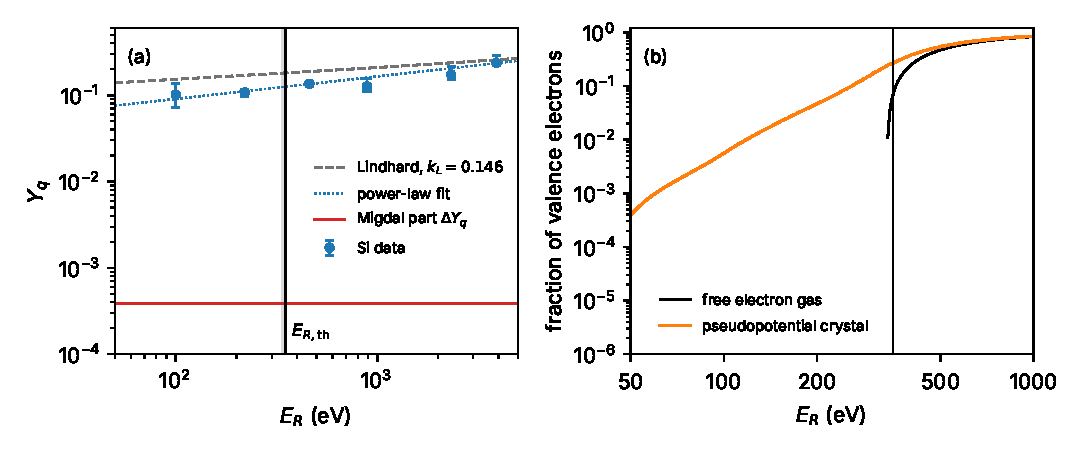
\includegraphics[width=\linewidth]{figures/ch19/fig19_2.pdf}
  \caption{The charge channel of silicon recoils. (a) Measured ionization yield $Y_q$ of silicon nuclear recoils (points: neutron scattering, total uncertainties, with \SI{3.8}{eV} per pair~\cite[Table~II]{albakry2023first}) against the recoil energy, with the power-law fit of the same work, $0.302(E_R/\SI{10}{keV})^{0.261}$ (dotted), and Lindhard's yield \cref{eq:16.6-lindhard} with $k_L = 0.146$ (dashed). Vertical line: the binary threshold $E_{R,\mathrm{th}} = \SI{352}{eV}$ of \cref{eq:19.2-Eth}; gray band: down to \SI{336}{eV}, the threshold with the $v_N^2$ term kept. Red: the part $\Delta Y_q^{\mathrm{Mig}}$ of the yield carried by Migdal electrons, \cref{eq:19.2-Ymig}, from the soft-limit spectrum of \cref{sec:12.3} converted to pairs by the silicon cascade of \cref{chap:18} with a uniform split of energy between electron and hole. (b) Fraction of valence electrons fast enough to be promoted across the gap $\Eg = \SI{1.17}{eV}$ by a head-on binary collision, $p \ge p_{\mathrm{min}}(E_R)$ of \cref{eq:19.2-pmin}: free electron gas of the valence density (black), which vanishes at \SI{336}{eV}, and the valence momentum density of the empirical pseudopotential model of \cref{sec:3.3} (four bands, $10^3$ points in the zone, plane waves to \SI{5.3}{\angstrom^{-1}}), whose smooth pseudo-orbitals understate the high-momentum tail; vertical line as in (a).}
  \label{fig:19-yield}
\end{figure}

\Cref{fig:19-yield}(a) shows the result. Between \SI{0.1}{keV} and \SI{3.9}{keV} the yield rises only from 0.10 to 0.24, and the two points below $E_{R,\mathrm{th}}$, at 0.10 and \SI{0.22}{keV}, agree with each other within their errors: there is no sign of an ionization threshold above \SI{100}{eV}. The Lindhard yield lies above the data at every energy below a keV, by a factor of 1.5 at \SI{100}{eV} (0.153 against 0.102) and by 1.4 at \SI{0.46}{keV}. Germanium, however, shows the opposite deviation. Recoils of \SI{254}{eV}, below its binary threshold of \SI{399}{eV}, give \SI{64 \pm 8}{eV} of electron-equivalent energy at \SI{77}{K}, a quenching factor of $\SI{25 \pm 3}{\percent}$ against Lindhard's \SI{14.3}{\percent}~\cite[abstract and Table~IV]{kavner2024measurement}.

The measured Fano factor of the nuclear-recoil charge, $F_{\mathrm{NR}} = \operatorname{Var}N_{\mathrm{eh}}/\langle N_{\mathrm{eh}}\rangle$, is $0.9^{+0.7}_{-0.4}$ at \SI{0.10}{keV}, $0.5^{+0.2}_{-0.1}$ at \SI{0.22}{keV} and $1.8^{+0.6}_{-0.5}$ at \SI{0.46}{keV}, and it grows to $8.4^{+2.4}_{-1.9}$ at \SI{3.91}{keV}~\cite[Table~II]{albakry2023first}, seventy times the electron-recoil value $F_{\mathrm{eh}} = 0.119$. Suppose the electronic energy $E_{\mathrm{el}}$ of a recoil were converted at a constant $\varepsilon_{\mathrm{eh}}$. The law of total variance would then give $\operatorname{Var}N_{\mathrm{eh}} = F_{\mathrm{eh}}\langle E_{\mathrm{el}}\rangle/\varepsilon_{\mathrm{eh}} + \operatorname{Var}E_{\mathrm{el}}/\varepsilon_{\mathrm{eh}}^2$, the cascade fluctuation at fixed $E_{\mathrm{el}}$ plus the fluctuation of $E_{\mathrm{el}}$ itself, so that
\begin{equation}
  F_{\mathrm{NR}} = F_{\mathrm{eh}} + \frac{\operatorname{Var}E_{\mathrm{el}}}{\varepsilon_{\mathrm{eh}}\langle E_{\mathrm{el}}\rangle} .
  \label{eq:19.2-FNR}
\end{equation}
At \SI{3.91}{keV}, with $\langle E_{\mathrm{el}}\rangle = Y_qE_R = \SI{923}{eV}$ and \SI{3.8}{eV} per pair, the measured $F_{\mathrm{NR}}$ requires a spread of \SI{170}{eV}, \SI{18}{\percent} of the mean: recoils of the same energy differ in how much of it reaches the electrons, because the sequence of collisions that each one makes is different. At \SI{100}{eV} the excitations lie near the gap and \cref{eq:19.2-FNR} no longer applies; there $F_{\mathrm{NR}}$ near one is what a few independent excitations of about one pair each would give.

\subsection{Migdal electrons in the measured yield}\label{sec:19.2-migdal}

The kick that starts the recoil already excites electrons, with the Migdal probability $P_{\mathrm{Mig}}$ of \cref{chap:12}. A neutron calibration measures the charge of real recoils, Migdal electrons included. The Migdal part of the yield is the integral \cref{eq:19.2-charge} taken over the soft-limit spectrum \cref{eq:12.3-soft}:
\begin{equation}
  \Delta Y_q^{\mathrm{Mig}} = \frac{\varepsilon_{\mathrm{eh}}}{E_R}\int\dd\omega_e\,\frac{\dd P_{\mathrm{Mig}}}{\dd\omega_e}\,\bar n(\omega_e) .
  \label{eq:19.2-Ymig}
\end{equation}
In the soft limit $\dd P_{\mathrm{Mig}}/\dd\omega_e$ is proportional to $v_N^2 = 2E_R/M_\kappa$, so the factor $1/E_R$ cancels and $\Delta Y_q^{\mathrm{Mig}}$ does not depend on the recoil energy. For silicon, the spectrum of \cref{sec:12.3} has $P_{\mathrm{Mig}} = 6.07\times10^{-3}$ at $E_R = \SI{100}{eV}$ with a mean electronic energy of \SI{5.97}{eV}. The energy-only cascade of \cref{chap:18} turns one such excitation into 1.69 pairs on average with a uniform split of the energy above the gap, or 1.92 if the electron takes all of it; the full-band cascade of \cref{sec:18.3-fullband} puts fewer events in the two-pair bin, and every Migdal excitation makes at least one pair. With \SI{3.8}{eV} per pair, the convention of the data,
\begin{equation*}
  \Delta Y_q^{\mathrm{Mig}} = \frac{\SI{3.8}{eV}}{\SI{100}{eV}}\times6.07\times10^{-3}\times1.69 = 3.9\times10^{-4} ,
\end{equation*}
and $4.4\times10^{-4}$ for the one-sided split; one pair per excitation gives the model-free lower edge $2.3\times10^{-4}$. The upper value is \SI{0.4}{\percent} of the measured yield at \SI{100}{eV} and \SI{0.3}{\percent} at \SI{0.46}{keV}. Both are soft-limit values, and the exact second-order bracket of \cref{sec:12.3-validity} lowers them, multiplying the Migdal probability by 0.93 at \SI{100}{eV} and by 0.62 at \SI{500}{eV}. The measured charge of silicon recoils at these energies is therefore almost entirely collisional.

A rate converted with the measured yield already contains the Migdal ionization (\cref{sec:12.1-counting}). Conversely, a computed yield must count the Migdal excitation at the kick and the collisional excitation after it, and nothing else. The trajectory calculation therefore starts after the kick, from the nuclear momentum and site distribution that the response hands over (\cref{sec:19.1}), and the lattice factor of the recoils that leave no Migdal electron has the weight $1 - P_{\mathrm{Mig}}$ of \cref{sec:12.1}, a \SI{0.6}{\percent} correction at \SI{100}{eV}. \Cref{sec:12.3-validity} met the boundary between the two channels from the Migdal side. Toward \SI{1}{keV} the second-order Migdal amplitude acquires a vanishing denominator, because the already moving nucleus ionizes the electrons on shell as a slow ion does, and that part belongs to the collisional channel of this section.

The balance between Migdal and collisional excitation shifts at low energy. The number of Migdal pairs per recoil falls in proportion to $E_R$. The collisional channel decreases for two reasons, fewer close collisions and the adiabatic suppression, whose factor $\ee^{-\xi_{\mathrm{M}}}$ falls from $1.1\times10^{-3}$ at \SI{100}{eV} to $2.6\times10^{-7}$ at \SI{20}{eV}, against a factor of five for the Migdal probability. If promotion at crossings follows the same trend, an estimate that only the kernel can confirm, the Migdal electrons become the dominant source of charge somewhere between a few tens of eV and \SI{100}{eV}, the recoil energies of dark matter below about \SI{0.44}{GeV}. That makes the Migdal rate of \cref{chap:12}, and not an extrapolated yield, the charge signal of the lightest nuclear-recoil searches.

\subsection{Open problems}\label{sec:19.2-open}

No calculation predicts the measured silicon yields and Fano factors below the binary threshold, or the germanium point at \SI{254}{eV}. The missing input is the close-collision kernel \cref{eq:19.2-kernel} for Si--Si and Ge--Ge collisions, with its exchange--correlation spread. Once it exists, the chain of partition trajectories, kernel and cascade also yields the probability of a recoil without charge, which sets the efficiency of a charge readout at the lowest recoil energies.
